%========================================================================= 
% SM11/2016 
% Mid Term Report IISER Thiruvananthapuram 
% Chapter 2
%=========================================================================

\chapter{SpinTaylorF2 waveform -- Overlap Study}

\label{chap:SpinTaylorF2 waveform}
\section{SpinTaylorF2 waveform}
The SpinTaylorF2 waveform~\cite{Lundgren2014} is a single spin, frequency domain
waveform that incorporates the effects of precession.  The waveform model
assumes one component of the binary to have negligible or zero spin; we will
therefore restrict our attention to NS-BH binaries, where the spin of the
neutron star is assumed to be neglible compared to that of the black hole.

Depending on the relative orientiation of the spin of the black hole to the
direction of the orbital angular momentum, the orbit of the NS-BH binary can
undergo precession over time. Concretly, if the spin of the black hole
$\mathbf{S}$ is misaligned with the orbital angular momentum $\mathbf{L}$ of the
binary, both $\mathbf{L}$ and $\mathbf{S}$ would precess about the total angular
momentum vector $\mathbf{J} = \mathbf{L} + \mathbf{S}$. Further, if $\mathbf{J}$
is not  small comapared to the orbital or spin angular momentum, the binary
undergoes simple precession~\cite{Apostolatos1994}, where total angular momentum
vector $\mathbf{J}$ remains nearly fixed during the inspiral, and $\mathbf{L}$
and $\mathbf{S}$ precesses about $\mathbf{J}$ with a uniform angular velocity. 
The SpinTaylorF2 waveform assumes simple precession, and breaks down in regions of 
parameter space where the assumption is no longer applicable. The expressions for 
evolution of $\mathbf{L}$ and $\mathbf{S}$ can be found in Eq.~(11) in~\cite{Apostolatos1994}.

\label{wf_compare}
\begin{figure}[t]
\includegraphics[width=\textwidth]{./images/TD_waveforms_comparison.pdf}
\caption{SpinTaylorF2 waveform in time domain. The upper plot clearly shows the modulations in the waveform amplitude due to precession compared 
to the non-preccesing waveform plotted below.}
\centering
\end{figure}

The precession of the orbital plane leads to modulations in the gravitational
wave amplitude and phase in the observer's frame of reference (see Fig.~1).
Interestingly, the precessing waveform in the observer's frame can be constructed  by
applying a time-dependent rotation to a non-precessing
waveform~\cite{Boyle2011}. The time-dependent rotation relates the observer's
frame to  reference to a frame that co-rotates with the precession of the
orbital angular momentum vector $\mathbf{L}$. The precessing waveform in the detector
frame $(h_{+},h_{\times})$ can then be expressed as a weighted sum of the co-
rotating frame amplitudes $\tilde{h}^{l,m}$ (see Eq. (3)
in~\cite{Lundgren2014}): 
\begin{equation}  
h_{+} + i h_{\times} = e^{-2 \psi}
\sum_{l,m,m^{\prime}} D^{l}_{m^{\prime},m} \left(\alpha, \beta, \gamma\right)
\tilde{h}^{l,m}(t){}_{-2}Y_{l,m^{\prime}}\left(\theta,\phi\right)e^{-i m \Phi}
\end{equation}  
where $D^{l}_{m^{\prime},m}$ is the Wigner rotation matrix of
SU2~\cite{Boyle2011}, and $\left(\alpha, \beta, \gamma\right)$ are the time-
dependent  Euler angles that relate the co-rotating frame to the observer's
frame. See~\cite{Lundgren2014} for complete definitions. 
Considering only the leading order $(l=2, |m| = 2)$ amplitude, 
we can express the above expression in frequency domain
using the stationary phase approximation~\cite{Lundgren2014}. Upon further simplification,
one arrives at the expression for SpinTaylorF2 waveform given by (see Eq. (12--13)
in~\cite{Lundgren2014}):
\begin{equation} 
\label{STF2_main}
h_{+}(f) = \dfrac{2\pi M_{c}^{2}}{D}\sqrt{\dfrac{5}{96\pi}}(\pi M f)^{-7/6}\sum_{m}z_{m}e^{i(\Psi - 2\zeta) + i m \alpha}
\end{equation}
where $D$ corresponds to the distance to the source, $M$ is the total mass and $M_{c}$ 
corresponds to chirp mass~\cite{Lundgren2014} of the binary. The expressions for $z_{m}, \alpha, \Psi$ and $\zeta$ 
can be found in~\cite{Lundgren2014}, we omit them for brevity. Each term in the summation in Eq.~(\ref{STF2_main}) 
represents a single sideband, corresponding to a particular value of $m$ ranging from $-2$ to $2$. Each sideband is 
therefore modulated in amplitude $(z_{m})$ and phase $(e^{i m \alpha})$ depending on the value of $m$. See Fig.~(\ref{wf_compare}), which 
compares time-domian plot of the waveform for a precessing and non-precessing case. In the non-precessing case, 
only the $m=2$ sideband has a non-zero amplitude; however, for a precessing system, all the sidebands
develop a non-zero amplitude. 

\section{Computation of Overlap and SNR}

Thus, one would expect that the single to noise ratio (SNR) from the total waveform would be sub-divided
into the SNR contribution from each of the individual sidebands in case of precession. 

\label{SNR}
\begin{figure}[h]
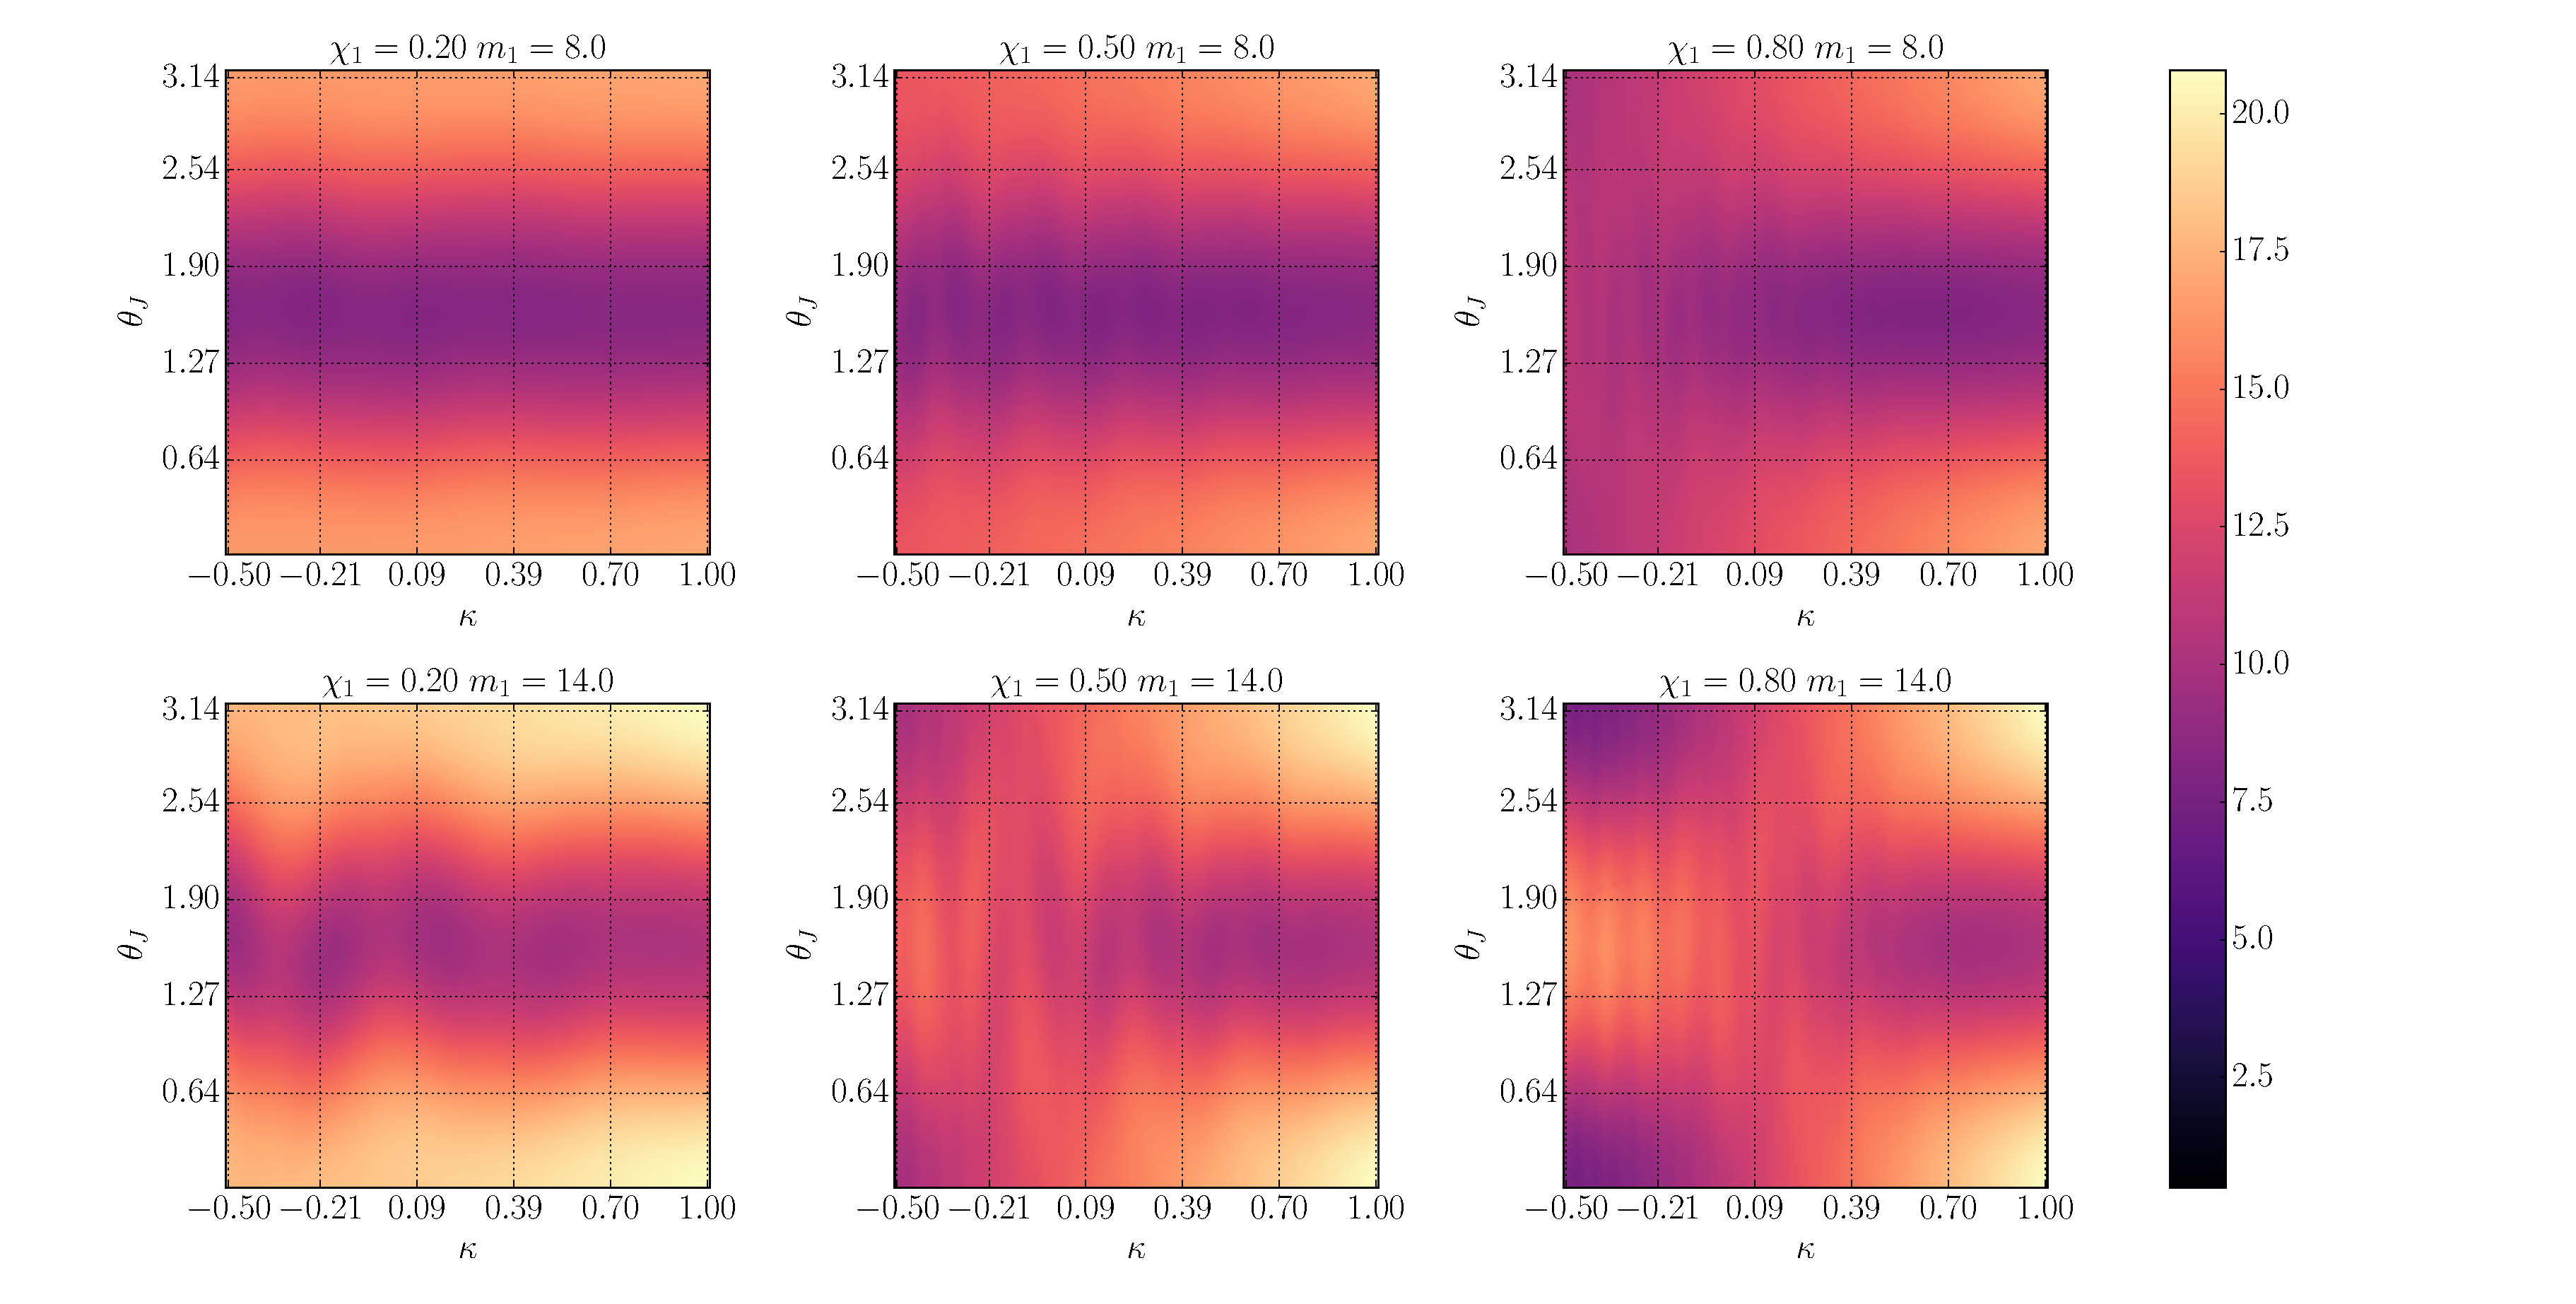
\includegraphics[width=0.7\textwidth]{./images/SNR_GRID_0F.pdf}
\centering
\caption{SpinTaylorF2 SNR plot. Each subplot corresponds to a particular value of mass and spin of the black hole, and each subplot shows the variation of SNR over $\kappa$ and $\theta_{J}$}.
\end{figure}

To investigate this further, we compute the SNR of 
full SpinTaylorF2 waveform. The signal-to-noise ratio (SNR) is computed as $(h|h)$, where $(h|h)$ is the noise-weighted scalar product defined as
\label{inner_product}
\begin{equation}
(a|b) = 4 Re \left[ \int_{f_{1}}^{f_{2}} df \dfrac{a^{*}(f)b(f)}{S_{n}(f)}\right].
\end{equation}
where $S_{n}(f)$ corresponds to the noise-power spectral density of the detector. Fig.~(\ref{SNR}) shows the SNR plot of the SpinTaylorF2 waveform 
over different regions of the parameter space. We plot the variation of SNR over $\theta_{J}$ which represents the orientation of the 
total angular momentum vector $\mathbf{L}$, and $\kappa$, which corresponds to the alignment of the spin vector 
$\mathbf{S}$ with the orbital angular momentum vector $\mathbf{L}$. We observe that the SNR is the highest in the region where $\theta_{J}$ corresponds to $0$ or $\pi$ which corresponds to the face-on or face-off region, and for $\kappa = 1$ which corresponds to the situation where $\mathbf{S}$ is along the direction of $\mathbf{L}$. To understand in which regions the sidebands contribute to the total SNR, we plot the overlap of each of the sidebands with the full waveform. The overlap between two frequency series $a(f)$ and $b(f)$ is given by
\begin{equation}
O_{ab} \equiv \dfrac{(a|b)}{\sqrt{(a|a)(b|b)}}
\end{equation}
The overlap of a particular sideband corresponds to the fractional SNR contribution of that sideband to the total SNR. We computed the overlaps for all the sidebands i.e. $m=-2$ to $m=2$ and found that the $m=0$ to $m=2$ modes are the dominant contributors to the total SNR of the full SpinTaylorF2 waveform. We also found that $m=0$ to $m=2$ dominate are different regions of the parameter space -- if the system is hihgly precessing, most of the SNR is captured by the $m=0$ sideband, and when the system is not precessing the $m=2$ has the dominant contribution to the SNR of the signal. Fig.~(3) shows the overlap plots for $m=2$ and $m=0$ sidebands with the full SpinTaylorF2 waveform. This suggests that one can use the sidebands -- which are computationally cheaper to generate than the full SpinTaylorF2 waveform -- to estimate parameters in the regions where their overlap with the full SpinTaylorF2 waveform is very high i.e. for precessing systems one can use the $m=0$ for parameter estimation since the maximum contribution to the SNR is coming from the $m=0$ mode when the system is precessing. This would allow for a massive reduction in computational cost associated with waveform generation. 

\section{Future Work}
Our future work would be to investigate this claim by performing parameter estimation with the full SpinTaylorF2 waveform and compare the results when a specific sideband is used in the appropriate region of parameter space (precessing or non-precessing) which would help us figure out how faithfully do we recover parameters if we use sidebands instead of the full waveform in parameter estimation.








